\section{Korišćenje generisanih stabala}
\label{sec:DesignPatterns}

Kako bi se stabla parsiranja i apstraktna sintaksička stabla mogla koristiti, potrebno je pružiti i uniformni interfejs za njihov obilazak. Postoje situacije kada se stablo obilazi sa ciljem izvršavanja operacija prilikom ulaska ili izlaska iz čvorova određenog tipa, ili pak sa ciljem izračunavanja neke konkretne vrednosti. Prilikom razvoja softvera se često nailazi na ovakve probleme i stoga su kreirana ponovno upotrebljiva rešenja za te probleme. 

\emph{Projektni obrasci} (engl. \emph{design patterns} \cite{DesignPatternsBook}, drugačije nazvani i \emph{projektni šabloni, uzorci}) predstavljaju opšte i ponovno upotrebljivo rešenje čestog problema, obično implementirani kroz koncepte objektno-orijentisanog programiranja. Svaki projektni obrazac ima četiri osnovna elementa:
\begin{itemize}
    \item ime --- ukratko opisuje problem, rešenje i posledice,
    \item problem --- opisuje slučaj u kome se obrazac koristi,
    \item rešenje --- opisuje elemente dizajna i odnos tih elemenata,
    \item posledice --- obuhvataju rezultate i ocene primena obrasca.
\end{itemize}

Projektne obrasce je moguće grupisati po situaciji u kojoj se mogu iskoristiti ili načinu na koji rešavaju zadati problem. Stoga je opšte prihvaćena podela na tri grupe:
\begin{itemize}
    \item \emph{gradivni obrasci} (engl. \emph{creational patterns}),
    \item \emph{strukturni obrasci} (engl. \emph{structural patterns}),
    \item \emph{obrasci ponašanja} (engl. \emph{behavioral patterns}).
\end{itemize}

Za potrebe ovog rada, projektni obrasci će se koristiti kao opšte prihvaćeno i programerski intuitivno rešenje određenih problema. Apstraktno sintaksičko stablo je primer upotrebe projektnog obrasca \emph{sastav}. Takođe, u kontekstu stabala parsiranja i apstraktnih sintaksičkih stabala, obrasci \emph{posmatrač} i \emph{posetilac} su od velikog značaja jer pružaju interfejs za obilazak takvih stabala. Ovi obrasci, opisani u narednim odeljcima, se koriste od strane ANTLR alata. Takođe, s obzirom da su ovi obrasci opšte-prihvaćeno rešenje za pružanje interfejsa obilaska stabala, biće korišćeni i u implementaciji opšte apstrakcije. U nastavku će zbog opisanih razloga biti opisani samo obrasci posmatrač i posetilac, dok zainteresovani čitalac može pročitati više u \cite{DesignPatternsBook}.

\subsection{Projektni obrazac "Sastav"}
\label{subsec:DesignPatternsComposite}

Projektni obrazac \emph{Sastav} je strukturni obrazac koji opisuje grupu objekata koji se tretiraju na isti način kao i individualna instanca istog tipa. Uloga sastava je da objekte organizuje u stablolike strukture kako bi se reprezentovale hijerarhije u kojima su neki elementi delovi a neki su celine. Sastav omogućava uniformno posmatranje individualnih objekata i čitavog sastava. Na slici \ref{fig:UMLComposite} se može videti UML dijagram \cite{UML} ovog obrasca. Za potrebe ovog rada, sastav će biti korišćen u implementaciji opšteg AST, s obzirom da je AST primer sastava.  

\begin{figure}[h!]
    \centering
    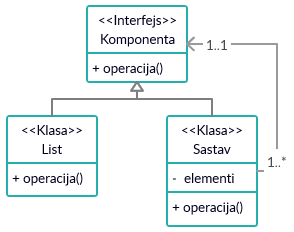
\includegraphics[scale=0.8]{images/design_composite.png}
    \caption{UML dijagram projektnog obrasca "Sastav".} 
    \label{fig:UMLComposite}
\end{figure}

\subsection{Projektni obrazac "Posmatrač"}
\label{subsec:DesignPatternsObserver}

Projektni obrazac \emph{Posmatrač} je obrazac ponašanja koji se koristi kada je potrebno definisati jedan-ka-više vezu između objekata tako da ukoliko jedan objekat promeni stanje (subjekat) svi zavisni objekti su obavešteni o izmeni i shodno ažurirani. Posmatrač predstavlja \emph{pogled} (engl. \emph{View}) u MVC (engl. \emph{Model-View-Controller}) arhitekturi. Na slici \ref{fig:UMLObserver} se može videti UML dijagram \cite{UML} ovog obrasca. Za potrebe ovog rada, primer upotrebe ovog obrasca može biti obilazak stablolike kolekcije (recimo stabla parsiranja) i obaveštavanje o nailasku na čvorove određenih tipova. Te informacije se dalje mogu iskoristiti za izračunavanja nad pomenutom strukturom ili generisanje novih struktura (recimo AST). 

\begin{figure}[h!]
\centering
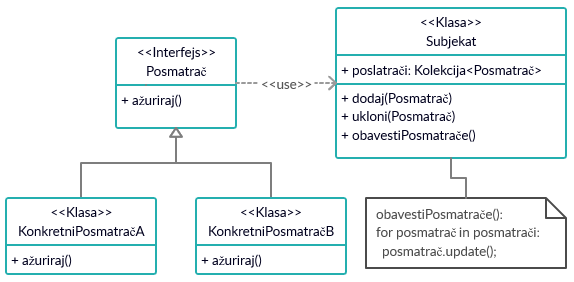
\includegraphics[scale=0.8]{images/design_observer.png}
\caption{UML dijagram projektnog obrasca "Posmatrač".}
\label{fig:UMLObserver}
\end{figure}

\subsection{Projektni obrazac "Posetilac"}
\label{subsec:DesignPatternsListener}

Projektni obrazac \emph{Posetilac} je obrazac ponašanja koji predstavlja operaciju koju je potrebno izvesti nad elementima objektne strukture. Posetilac omogućava definisanje nove operacije bez izmena klasa elemenata nad kojima operiše. Operacija koja će se izvesti zavisi od imena zahteva, tipa posetioca i tipa elementa kog posećuje. Na slici \ref{fig:UMLVisitor} se može videti UML dijagram \cite{UML} ovog obrasca. Za potrebe ovog rada, primer upotrebe ovog obrasca može biti prikupljanje informacija o kolekciji stablolike strukture (recimo stablo parsiranja) i korišćenje istih za neko izračunavanje ili generisanje novih struktura (recimo AST). 

\begin{figure}[h!]
    \centering
    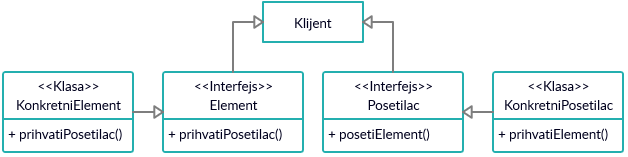
\includegraphics[scale=0.8]{images/design_visitor.png}
    \caption{UML dijagram projektnog obrasca "Posetilac".} 
    \label{fig:UMLVisitor}
\end{figure}